\section{Evaluation}
We first integrate SchemaLine into an existing visual analytics system, and then evaluate its usefulness in exploring temporal relationship of the sensemaking task.

\subsection{Application}
% Overview of INVISQUE
We integrate SchemaLine into INVISQUE~\cite{Wong2011} -- a visualization system designed for interactive exploration of text documents. INVISQUE provides full-text search and organizes search results in a two-dimensional spatial canvas, with each dimension representing a customized attribute. For example, it may be useful to order academic articles horizontally by publication date and vertically by citation count. Search results from a keyword are shown as a cluster of \emph{index-cards}, each representing a document with selected information such as publication title, date, keywords and authors. \autoref{fig:invisque} shows a screenshot of INVISQUE.

\begin{figure}[!htb]
	\centering
	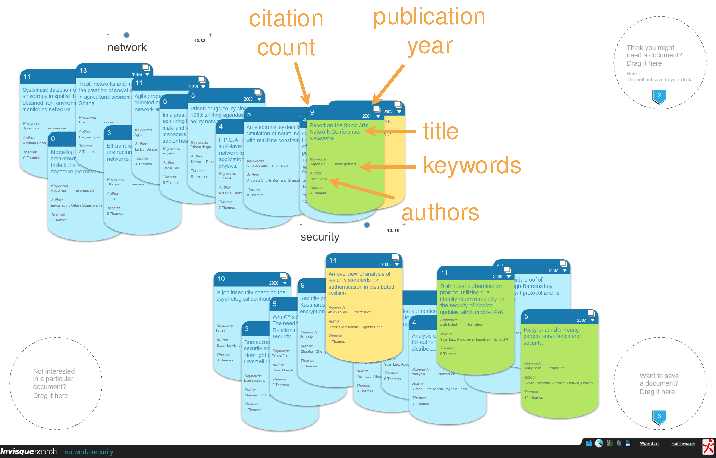
\includegraphics[width=\linewidth]{invisque}
	\caption{INVISQUE interface. It shows two sets of search results for ``network'' and ``security'' from a publication dataset.}
	\label{fig:invisque}
\end{figure}

% Integration
We add an \emph{annotation} feature enabling users to record their thoughts while reading documents. These annotations are important to users, thus are also displayed on the index-cards. We choose them as the input \emph{events} of the SchemaLine visualization. SchemaLine is placed at the bottom of INVISQUE. After the user makes a note, or annotation, it is immediately added to SchemaLine as a new event. Double clicking on an event will open the document containing that note as an index-card, enabling the user to quickly reexamine the original information resource.

% Attribute mapping
The \emph{temporal information} of documents, such as ``publication date'', is initially assigned to that of events, and can be changed later by users to match the correct meaning. This feature is useful because the report date is not necessary the same as the date when the event actually occurred. For example, a news article can write about a bomb attack in some city yesterday. The user can perform this change by dragging an event with the right mouse button along the time axis and dropping it at the desired date. 

The \emph{label} of an event simply maps to the content of an annotation itself. In INVISQUE, we color code search keywords that contain annotated documents, and use them as \emph{categories} for events. Because a document can be returned from different searches, it can also contain multiple categories. This mapping provides context for the annotations: what did I search for (the original keyword) and what are other related concepts (other search keywords returning the same document)? This context may help users to discover interesting patterns through their annotations. \autoref{fig:invisque-schemaline} shows a screenshot of INVISQUE with SchemaLine integrated.

\begin{figure}[!htb]
	\centering
	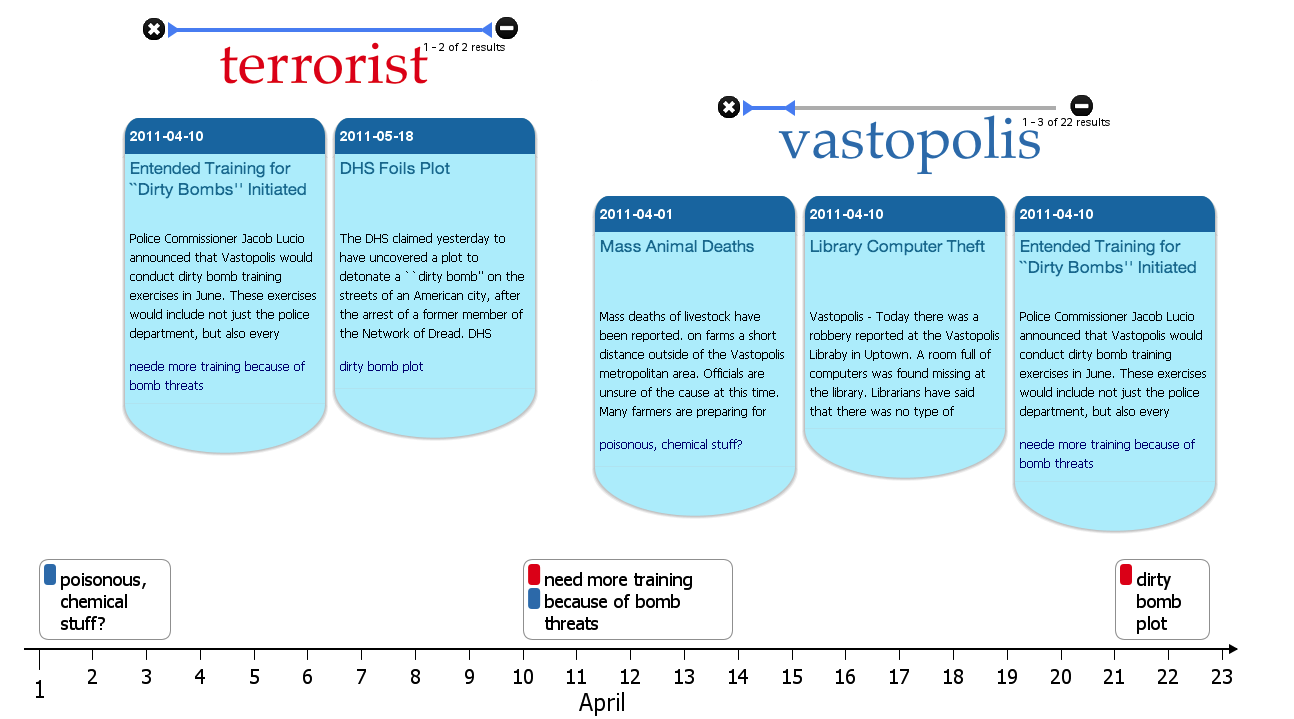
\includegraphics[width=\linewidth]{invisque-schemaline}
	\caption{INVISQUE with SchemaLine at the bottom. The timeline consists of three events, which are user taken notes. Color coded categories of events indicate keywords that were searched for.}
	\label{fig:invisque-schemaline}
\end{figure}

\subsection{Case Study}

\subsubsection{Design}

\paragraph{Method}
Evaluating the usefulness of SchemaLine in supporting sensemaking can be categorized as \emph{evaluating visual data analysis and reasoning} -- one of the seven scenarios in evaluating information visualization proposed by Lam~et~al.~\cite{Lam2012}. The goal of this type of evaluation is to explore whether and how a visualization tool supports participants to make sense and generate relevant knowledge in a domain. During solving sensemaking tasks, the participants may employ various strategies. Their processes and outcomes are highly context-sensitive, making it difficult to quantify and compare their performance. Therefore, sensemaking evaluations are typically case studies with realistic datasets and domain experts as participants. We conducted a case study to explore how SchemaLine supports users to solve a task, focusing on how it enables them to perform sensemaking activities in the Data--Frame model.

\paragraph{Task}
We used the task from Mini Challenge 3 of the IEEE VAST Challenge 2011~\footnote{\url{http://hcil2.cs.umd.edu/newvarepository/VAST Challenge 2011/challenges/MC3 - Investigation into Terrorist Activity/}}, which requires the participants to identify any potential criminal activities from the given dataset. We chose this task because it resembles a real task in a domain (intelligence analysis), and the solution was provided and well-tested by the community. INVISQUE with SchemaLine integrated was used in the study. 

\paragraph{Participants and Procedure}
We were unable to recruit real intelligence analysts for the study. Instead, we recruited three graduate students with different backgrounds:  one in visual analytics (surrogate for visualization expert -- \textbf{P1}), one in law (surrogate for domain expert -- \textbf{P2}), and one in networking (neutral background -- \textbf{P3}). After being introduced features of INVISQUE and SchemaLine, participants had a chance to practice with a trial sensemaking task for 15 minutes. The main task was followed and lasts for one hour. The participants were asked to report the criminal activities they had discovered with the supporting evidence. Semi-structured interviews were followed to gain deeper understanding of the processes.

\paragraph{Pilot Tests}
We conducted two pilot tests to assess the study design. The original dataset contains more than four thousand news reports, many of which have more than 500 words. In the pilots, both participants failed to find any answers after one and a half hours. Most time was spent on reading long but irrelevant documents. The reason could be INVISQUE does not support text-mining features such as entity extraction, which is crucial in analyzing a large document collection. The goal of the evaluation was to assess how SchemaLine can provide additional sensemaking support to INVISQUE rather than assessing INVISQUE itself. Therefore, in the main study, we removed all irrelevant documents that are not part of the ground truth, which actually added by the organizers to challenge contestants. The new dataset contains 36 documents including five criminal activities:  food poisoning (13 documents), hacking (3), dirty bomb (6), arms trafficking (4), and money laundering (3). Other documents are isolated cases and are not considered as correct answers. We expected that  participants could complete the task within a reasonable amount of time, without affecting the goal of the study. 

\subsubsection{Results and Discussion}
We first summarize the three sessions and present our findings next.

\paragraph{Participant 1}
\textbf{P1} began searching for ``bomb'', examined the search results, and searched for  a refined keyword ``dirty bomb''. He took notes in three documents and then linked these notes together (\emph{connect data and a frame}). He then searched for ``Network of Dread'', which was mentioned in one document as the author of the dirty bomb attack. He took a note in the new returned document and dropped it onto the ``dirty bomb'' colored schema (\emph{elaborate the frame}). While investigating, he encountered an article about a man carrying a frozen turkey having wires coming out of it, which was suspected as a bomb. At first, he dropped the ``turkey bomb'' note onto the ``dirty bomb'' schema. Then, he wondered whether it is a real bomb. After thinking for a while, he removed it out of the schema (\emph{preserve the frame}). \textbf{P1} found the ``dirty bomb'' attack with 4/6 correct pieces of evidence. \textbf{P1} took many notes in documents related to the ``food poisoning'' case; however he could not link them together because he said that ``I'm not familiar with bio-attack so I couldn't think of it as a threat''. 

\paragraph{Participant 2}
\textbf{P2} took an overview step before searching. He quickly looked at all 36 document titles to have a glimpse of the dataset as well as to detect potential search keywords. He began searching ``animal deaths'', read the results, took notes and grouped them together (\emph{connect data and a frame}). He was happy with the evidence he found for that crime and switched to read another interesting article ``Library Computer Left'' he came across. From that, he searched for several related terms such as ``computer'' and ``hackers''. He figured out that a group called ``F-alliance'' stole computers from the library and attempted to hack a bank. He dropped a ``computer stolen'' note on top of a ``bank hacking'' note to form a new explanation for the case (\emph{connect data and a frame}). He found another article related to hacking but he said ``I won't drop it to this group because it's just an announcement from the government about potential threats'' (\emph{preserve the frame}). During further investigation, he created another group of notes related to ``bioterrorism'' and ``Prof. Patino''. Then, when figuring out that the reason of the mass deaths is a spore-forming microbe, which is also mentioned in Prof. Patino's talk, he dropped that new group onto the ``animal deaths'' group to combine all notes together because he thought that they are related (\emph{merge frames}). Observing the order of events in the new group on the timeline, he said ``The equipment of Patino was stolen after the animal deaths report, so they couldn't be used in that case. This is the group of a potential threat in using bioterrorism'' (\emph{elaborate the frame}). \textbf{P2} found the ``hacking'' case with 2/3 correct pieces of evidence and the ``food poisoning'' case with 9/13 correct pieces of evidence. \autoref{fig:evaluation} shows the computer screen of \textbf{P2} when he reported his findings.

\begin{figure*}[!htb]
	\centering
	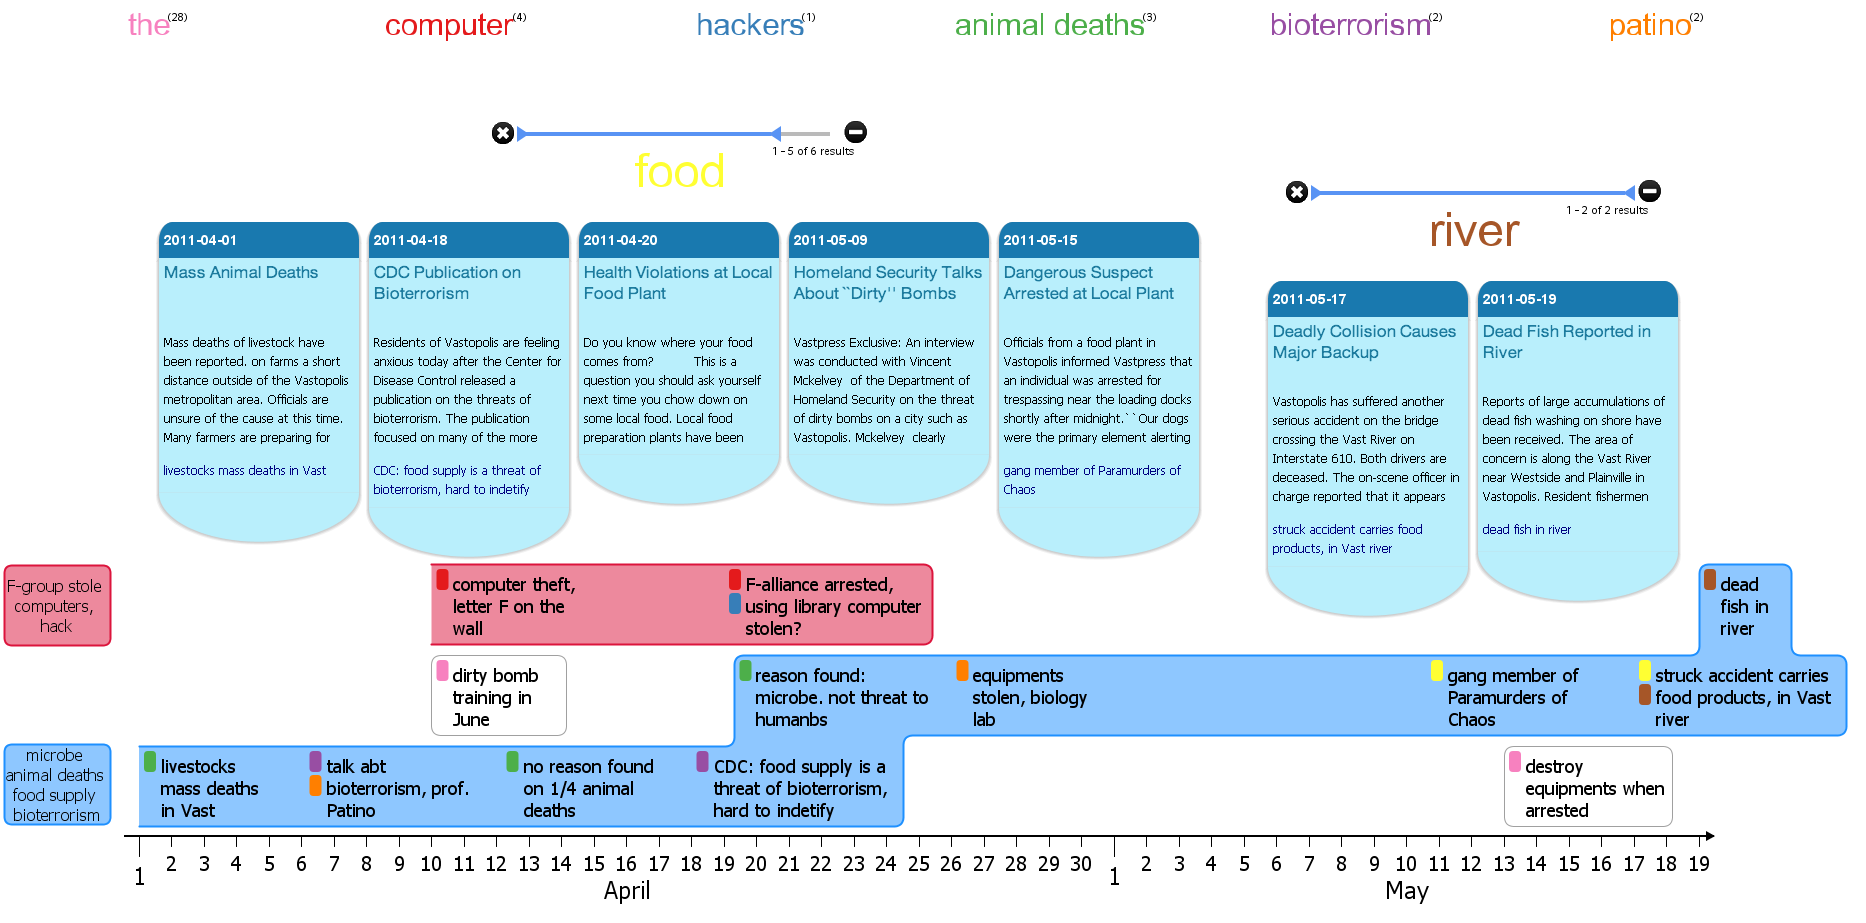
\includegraphics[width=\linewidth]{evaluation}
	\caption{Final screen of participant \textbf{P2}. Top: a trail of his keyword searches, collapsed after being read. Middle: search results in index-card metaphor. Bottom: two schemas containing notes as supporting evidence of criminal activities he found.}
	\label{fig:evaluation}
\end{figure*}

\paragraph{Participant 3}
\textbf{P3} searched for a few keywords related to criminal activities before examining the search results such as ``bomb'', ``terrorism'', ``money'' and ``hack''. He took and group notes about ``money laundering'' together (\emph{connect data and a frame}). Then, he read articles from ``terrorism'' search results. He followed the article content to search for relevant information such as ``Paramurderers of Chaos'' -- a terrorist group. During further investigation, similar to \textbf{P2}, he also combined two groups of notes -- ``Paramurderers of Chaos'' and ``food supply'' -- together when discovering evidence linking the two groups (\emph{merge frames}). When representing his findings, he shared that SchemaLine prompted him to look for missing information. ``I noticed the gap between these two events [pointing to the timeline]; then I knew I probably missed something there'' (\emph{question the frame}). \textbf{P3} found the ``food poisoning'' case with 6/13 correct pieces of evidence, and a perfect 3/3 pieces of evidence in the ``money laundering'' case. 

\paragraph{Discussion}
% All take notes, build schemas
Three participants applied different sensemaking strategies. \textbf{P1} started with a potential search keyword for criminal activities and kept following the search results. \textbf{P2} scanned the titles of all documents to have an overview of the dataset first. \textbf{P3} planned ahead what he wanted to search for and sequentially executed it. However, all of them extensively took notes and constructed frames to organize them. These frames presented various forms: a concept (bioterrorism), a criminal activity (dirty bomb), a person (Prof. Patino) and a group of people (Paramurderers of Chaos). All participants also employ a variety of sensemaking activities described in the Data--Frame model, supported through fluid interaction in SchemaLine.

% temporal sensemaking
All participants appreciated the automatic addition of user notes to the timeline. \textbf{P1} thought that he would have a problem if the system did not support that: ``I can remember what happened but it was difficult to remember when they happened''. They found that the chronological order of events helps them to construct the story lines. \textbf{P2} shared that he read the news about the robbery at Vastopolis university and the Prof. Patino's talk about bioterrorism. However, he did not have any insight at that time. When looking at his two notes on the timeline, he thought that the extremely expensive equipment in Prof. Patino's lab could be the reason of the robbery. 

% intuitive interface & presentation
All participants commented that the interaction between data and frame is very intuitive. \textbf{P1} even said ``I think I don't even need training and still can figure out how it works''. \textbf{P3} liked the transition effect when adding or removing notes because ``it helped me to understand what is going on''. All participants were confident when presenting their analyses. \textbf{P3} even opened the original document (double-clicking on the note) several times to highlight the relevant text. He said that the connection between the note and the containing document enabled him to quickly find the information source when needed.